 
In this chapter, we discuss different domains and concepts applied in our proposal, including compilers, code generators, optimizations and non-functional requirements.
The objective of this chapter is to give a brief introduction to these concerns, used throughout the thesis. This introduction aims at providing a better understanding of the background and context in which our work takes place, as well as the terminology and concepts presented in the next chapters.

The chapter is structured as follows:
\section{From classical software development to generative programming}
%context
The history of software development shows a continuous increase of complexity in several aspects of the software development process\cite{betz2011improving}. 
%Diversity
In fact, modern software systems rely nowadays on a highly heterogeneous and dynamic interconnection of platforms and devices that provide a wide diversity of capabilities and services. These heterogeneous services may run in different environments ranging from cloud servers with virtually unlimited resources down to resource-constraint devices with only a few KB of RAM. Effectively developing software artifacts for multiple target platforms and hardware technologies is then becoming increasingly important and developing software. 
%problem
Furthermore, the increasing relevance of software in general and the higher demand in quality and performance contribute to the complexity of software development. In comparison to the classical approach where software development was carried out manually, today’s modern development requires more automatic and flexible approaches to handle this given complexity.
Hence, more generic tools, methods and techniques are applied in order to keep the software development process as easy as possible for testing and maintenance and to handle the different requirements in a satisfyingly and efficient manner.
%GP
As a consequence, generative programming (GP) techniques are increasingly applied to automatically generate and reuse software artifacts.
%GP definition
Generative programming \textit{is a software engineering paradigm based on modeling software families such that, given a particular requirements specification, a highly customized and optimized intermediate or end-product can be automatically manufactured on demand from elementary, reusable implementation components by means of configuration knowledge}\cite{Czarnecki:2000:GPM:345203}. 
This paradigm offers the promise of moving from "one-of-a-kind" software systems to the semi-automated manufacture of wide diversity of software.

%figure
Generative software engineering consists on using higher-level programming techniques such as meta-programming, modeling, DSL, etc in order to automatically generate efficient code for the the target software platform. 
In principle a software development process can be seen as a mapping between a problem space and a solution space\cite{czarnecki2005overview} (see Figure 2.1). 

%problem space
\textbf{The problem space} is a set of domain-specific abstractions that can be used by application engineers to express their needs and specify the desired system behavior. This space is generally defined  as DSLs or high-level models. 

%solution space
\textbf{The solution space}, on the other hand, consists of a set of implementation components, which can be composed to create system implementations (for example, the generation of platform-specific software components written using general-purpose languages such as Java, c++, etc).

%mapping
\textbf{the configuration knowledge} constitutes the mapping between both spaces. It takes a specification as input and returns the corresponding implementation as output. It defines the construction rules (i.e., the translation rules to apply in order to translate the input model/DSL into specific implementation components) and optimizations (i.e., optimization can be applied during code generation to enhance some of the non-functional properties such as execution speed). It defines also the dependencies and settings among the domain specific concepts and features.


%GP advantages
These schema integrates several powerful concepts from Model Driven Engineering (MDE), such as domain-specific languages, feature modeling, generators, components, and software architecture. 

Some commonly benefits of such software developing architecture are:
\begin{itemize}
\item It reduces the amount of re-engineering/maintenance caused by specification requirements
\item It facilitates the reuse of components/parts of the system
\item It increases the decomposition and modularization of the system
\item It handles the heterogeneity of target software platforms by automatically generating code
\end{itemize}
\begin{figure}[h]
	\center
	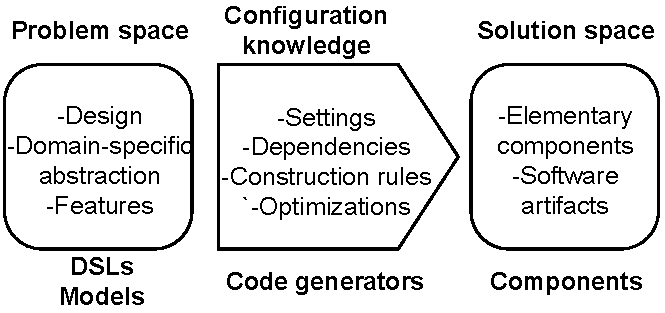
\includegraphics[scale=0.65]{Background/fig/GDM.pdf}
	\caption{Overview of the Docker-based testing architecture}
\end{figure}

\textbf{Among the main contributions of this thesis is to verify the correct mapping between the problem space and solution space. In other words, we would evaluate the impact of applied configurations during code transformation on the resource usage requirements.
}

In the following section, we present a general overview of the abstract software development tool chain and the main actors that are involved.

\section{Software development tool chain overview}
The process of generative software development involves many different technologies. In this section, we describe in more details the different activities and actors involved to transform high-level specification into executable programs and that from design time to runtime. 
Figure 2.2 review the different steps of this chain. We distinguish four main tasks: 
\begin{itemize}
\item \textit{Software design:} As part of the generative programming process, the first step consists on representing the system abstraction. Thus, software designers define, at design time, software’s behavior using domain models or Domain-Specific Models (DSMs). A DSM is a system of abstractions that describes selected aspects of a sphere of knowledge and real-world concepts pertinent to the domain that need to be modeled in software. These models are specified using a high-level abstract languages (DSLs). Domain-specific languages (DSLs) improve programmer productivity by providing high-level abstractions for the development of applications in a particular domain.

\item \textit{Code generation:} Software developers use model-driven techniques in order to generate automatically code. Thus, instead of focusing their efforts on constructing code, they build models and, in particular, create model transformations that transform these models into new models or code. 

TOFINISH
\item \textit{Software development:}
TODO
\item \textit{Compilation:}
TODO
\end{itemize} 
.
%\begin{figure}[h]
%\center
%	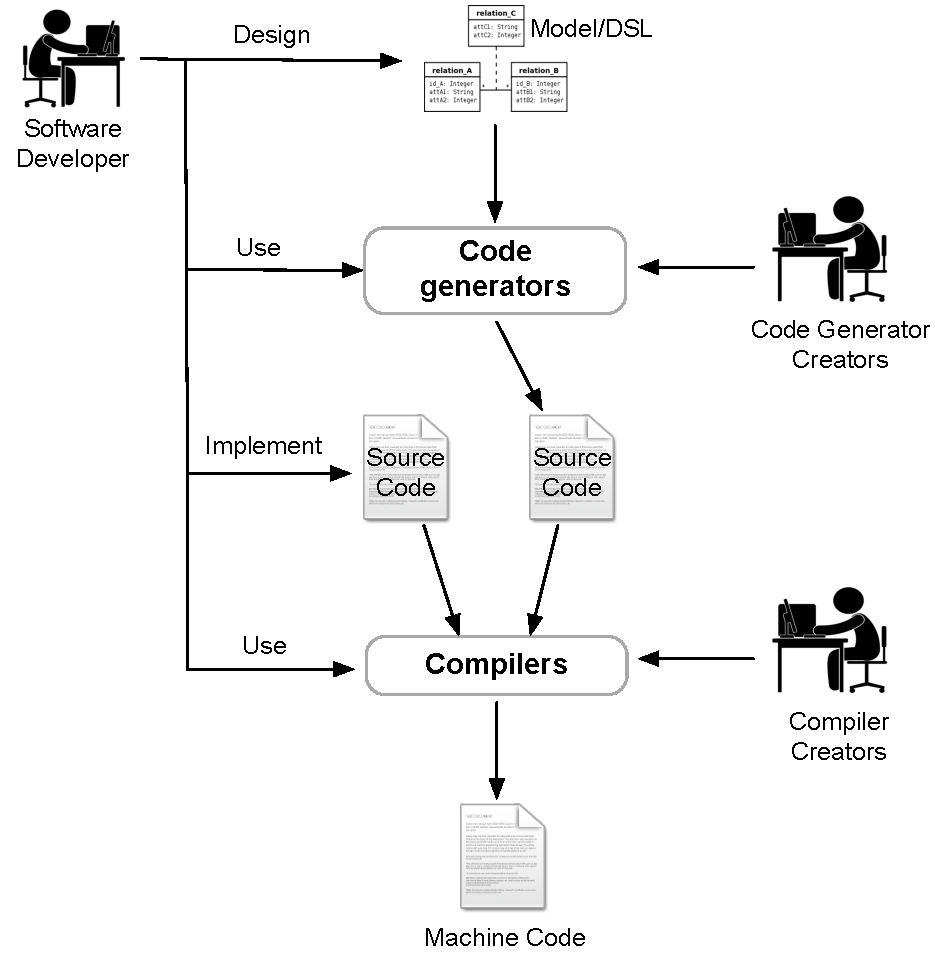
\includegraphics[scale=0.65]{Background/fig/background_overview.pdf}
%	\caption{Overview of the Docker-based testing architecture}
%\end{figure}
\begin{figure}[h]
\center
	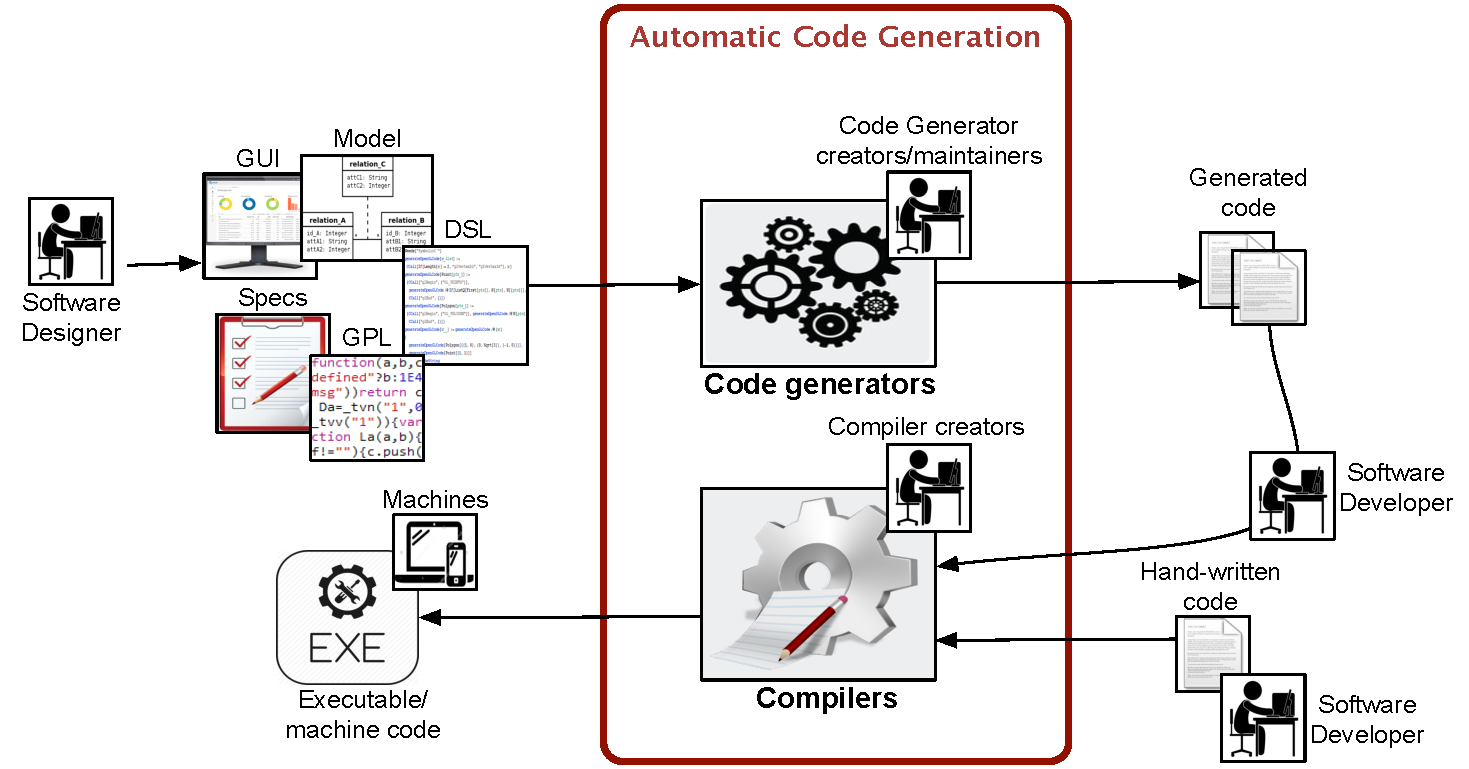
\includegraphics[scale=0.65]{Background/fig/background_overview2.pdf}
	\caption{Overview of the Docker-based testing architecture}
\end{figure}


\section{Code generators}
The main goal of generators is to produce software systems from higher-level specifications. Generators bridge the wide gap between the high-level system description and the executable. Generators are based on domain-specific models which define the semantics of the system specification language and also contain the knowledge of how to produce efficient implementations[REF]. 
We distinguish two major types of code generators: rule-based model-to-model transformation languages (such as ATL) and template-based model-to-text transformation languages (such as Acceleo) to translate high-level system specifications into executable code and scripts.
\subsection{Complexity}
The complexity of code generators remains on the transformation rules and code generation process. In fact, code generators can be difficult to understand since they are typically composed of numerous elements, whose complex interdependencies pose important challenges for developers performing design, implementation, and maintenance tasks. 
Given the complexity and heterogeneity of the technologies involved in a code generator, developers who are trying to inspect and understand the code-generation process have to deal with numerous different artifacts. As an example, in a code-generator maintenance scenario, a developer might need to find all chained model-to-model and model-to-text transformation bindings, that originate a buggy line of code to fix it. This task is error prone when done manually. We believe that flexible traceability tools are needed to collect and visualize information about the architecture and operational mechanics of code generators, to reduce the challenges that developers face during their life-cycle.[ref W]

Moreover, the generated code has to meet certain performance requirements (e.g. execution speed, response time, memory consumption, utilization of resources, etc.). The challenge is that the structure of the specification is usually very different from the structure of the implementation: there is no simple one-to-one correspondence between the concepts in the specification and the concepts in the implementation. 
Efficient implementations are then computed at generation time by applying domain-specific optimizations and replacing, merging, adding, and removing components.

\textbf{Challenge}: Fully automatic program synthesis offers many gains over traditional software development methods. e.g., speed of development, increased adaptability and reliability. But code generators are complex pieces of software themselves that may contain bugs.
\begin{itemize}
\item Can you trust the code-generator?
\item How can the correctness of the generated code be verified?
\end{itemize}
\subsection{Software-platform heterogeneity}
The key concept of code generators is to produce code in a general-purpose language, such as Java or C++, that can be compiled and executed. Target execution platforms of the generated code are heterogeneous and diverse.
for example, although Android provides Java syntax, it uses its own Google libraries and creates byte code that will not run on the standard JVM (Java Virtual Machine). This means that consumers are carrying devices that support different programming languages and developers will usually need to create multiple clients in this heterogeneous environment.
\begin{figure}[h]
	\center
	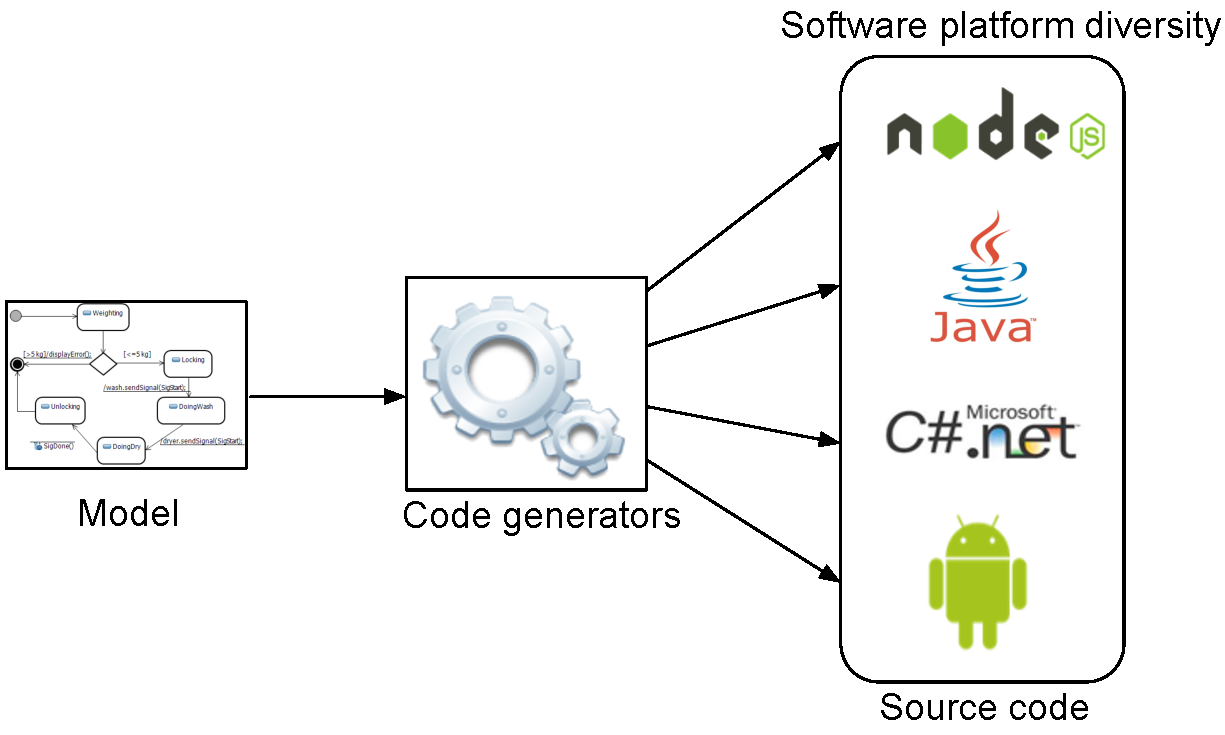
\includegraphics[scale=0.65]{Background/fig/software-diversity.pdf}
	\caption{Overview of the Docker-based testing architecture}
\end{figure}
\section{Compilers}
\subsection{Complexity}
Modern compilers implement a number of optimizations. Each optimization tries to improve the performance of certain target applications. Improvement of source code programs in terms of performance can refer to several different non-functional properties of the produced code such as code size, resource or energy consumption, execution time, among others~\cite{almagor2004finding,pan2006fast}.
Testing non-functional properties is more challenging 
Thus, the determination of optimal settings of compiler optimizations has been identified as a major problem because compilers may have a huge number of potential optimization combinations, making it hard and time-consuming for software developers to find/construct the sequence of optimizations that satisfies user specific key objectives and criteria. It also requires a comprehensive understanding of the underlying system architecture, the target application, and the available optimizations of the compiler.
\subsection{Hardware-platform heterogeneity}
\begin{figure}[h]
	\center
	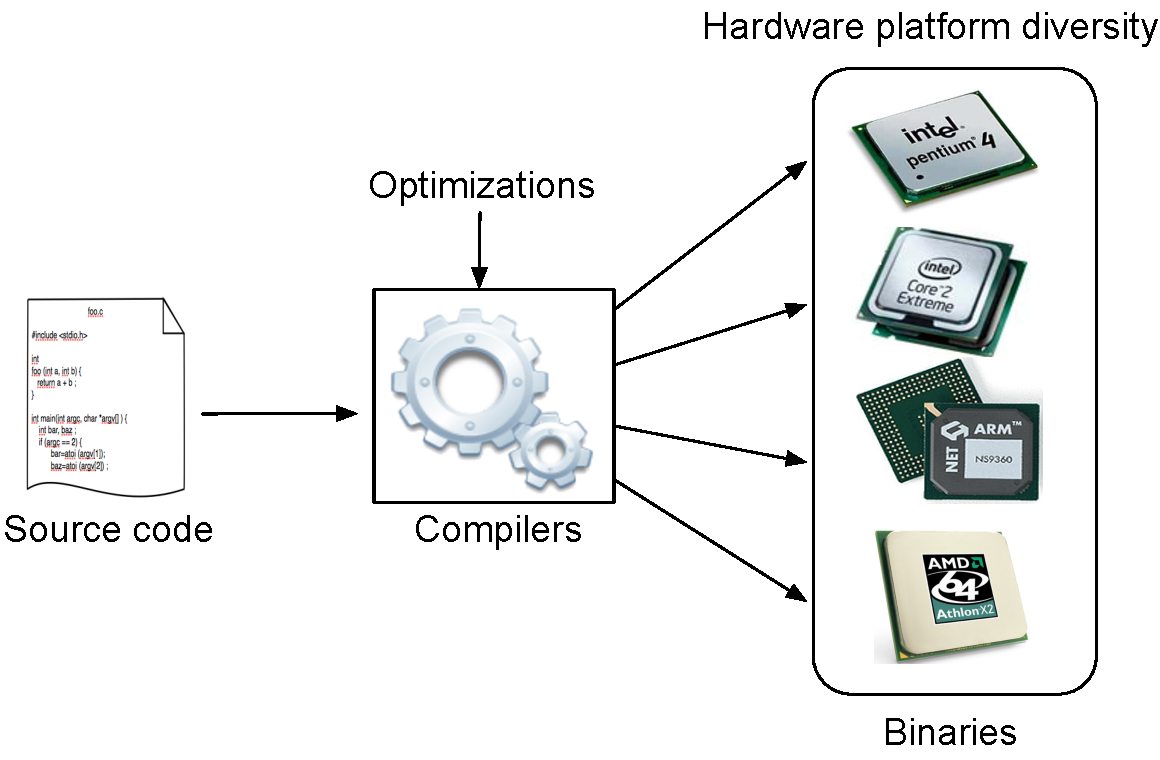
\includegraphics[scale=0.65]{Background/fig/hardware-diversity.pdf}
	\caption{Overview of the Docker-based testing architecture}
\end{figure}
Generally, software developers use different compilers in order to compile their source code program and execute it on top of a board range target platforms and processors such as arm, intel, amd processors. 

Compilers can be classified depending on the platform on which their generated code executes. This is known as the target platform.
A native compiler is one which output is intended to directly run on the same type of processor architecture and operating system that the compiler itself runs on. In the counter part, the output of a cross compiler is designed to run on a different platform. Cross compilers are often used when developing software for embedded systems that are not intended to support a software development environment.

Given the complexity of new emerging processors architecture, rapidly evolving hardware and compiler options, it is not easy to deliver satisfactory levels of performance on modern processors.


Some of the questions that developers have to answer when facing Hardware diversity which optimizations are applied by compiler users in order to satisfy the non-functional properties of a broad range of programs and hardware architectures such as energy consumption, execution time, etc. 






%\section{Compilers and Code generators non-functional testing}
\subsection{Problems that still remain}
\begin{itemize}
	\item Resource usage monitoring of generated code: Due to the software and hardware heterogeneity, monitoring the resource usage of each execution platform is still challenging and time-consuming. 
	\item Auto-tuning compilers:
	\item Detecting bugs in code generators: 
%\subsection{Resource usage monitoring}
\end{itemize}
